\section{Implementation and Runtime}
\label{sec:runtime}
In this section we discuss our extensions for the MapReduce programming model and show the major changes to runtime of \myds. 
Then we describe our design how to support pipelining of Map and Reduce phase (Section 4.2.1).
The implementation of intermediate buffer between Map and Reduce phase will be given in Section 4.2.2.
Finally, we defer performance results to Section 5.



\subsection{Execution flow}
\begin{figure}[!h!t]  
    \centering
    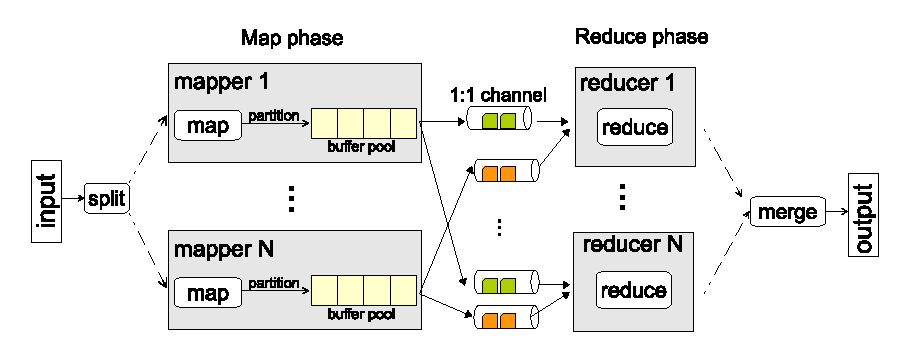
\includegraphics[width=0.45\textwidth]{eps/dmr_workflow.eps}
    \caption{The workflow of \myds}
    \label{fig:dmr:workflow}
\end{figure}

%不同与Phoenix,DMR将任务队列静态的划分给每个map worker,这样做的好处是,可以避免多个map worker对对任务队列操作从而产生锁的开销。
The implementation of MapReduce in  \myds is similar to that of in Phoenix. 
There is a single master worker managing a number of slave workers. Unlike Phoenix,  a worker in \myds is handled by a \myth thread rather than a Pthread thead.
Figure \ref{fig:dmr:workflow} illustrates the workflow of \myds, including three main phases: map, reduce and merge. 
At the beginning,  the input data is divided into some tasks by a split function, and then these tasks are pushed  into a task queue. 
%On multi-core CPUs, a worker is handled by one thread, which is a \myth thread in \myds.
%A worker usually needs to process multiple input elements. 
%Thus the map function is applied to the input elements one by one. 
%Such an operation of applying the map function for an input element is 
%called a map operation. 
%Each map operation produces intermediate key-value pairs. 
%Then a partition function is applied to these key-value pairs. 
%Then in the reduce phase, each reduce operation
%applies the reduce function to a set of intermediate pairs
%with the same key. 
Then workers in Map phase will get these tasks from the task queue and apply the map function to the tasks.
The intermediate key-value pairs produced by the map worker will be inserted into a local buffer.
When this local buffer is full, the map worker will send the intermediate data of the buffer to a one-to-one channel.
After that, the reduce worker can receive this data from the channel and invoke reduce function to aggregate them with the same key.  
Finally the results from multiple reduce workers are merged and output.

Compared with existing work, our \myds takes two main strategies to improve its scalability and performance.
On the one hand, a worker in \myds is implemented as a \myth thread instead of a shared-memory thread.
Therefore, threads in the isolated address space can avoid contending on a single per-process lock, which has introduced in Section 3.2.
On the other hand, the producer-consumer model in Section 3.2 is used to pipeline Map and Reduce phase,
i.e., the map worker as a producer send key-value pairs to the channel and  the reduce worker as a consumer will receive the key-value pairs from the channel. 
Once the reduce workers receive these key-value pairs, it will invoke the reduce function to work with no need for waiting all workers in Map phase finished.
%As a result, \myds breaks the barrier in Phoenix.

%The map phase reads the task’s split from task queue,
%parses it into key-value pairs, and applies
%the map function to each record.
%Intermediate keys are assigned
%to reducers by applying a partitioning function
%A spill of the in-memory buffer involves first sorting
%the records in the buffer by partition number and then by
%key.

%After receiving its partition from all map outputs, the
%reduce task enters the sort phase. The map output for
%each partition is already sorted by the reduce key. The
%reduce task merges these runs together to produce a sin-
%gle run that is sorted by key. The task then enters the
%reduce phase, in which it invokes the user-defined reduce
%function for each distinct key in sorted order, passing it
%the associated list of values.
%
%We addressed these issues by buffering the mapper output until
%it reaches a certain record threshold.
%When the record threshold isreached, 
%the mapper sends the output to a reducer. 
%Next, Reducer receives its partition from all map, 
%and enters the sort phase.
%将之前对combiner和merge阶段的特征进行简单的总结
{\bf Combiner.}
There is a optional \code{Combiner} operation, which is a local aggregation in Map phase, can maximally reduce memory pressure caused by the intermediate key-value storage.
In addition, the \code{Combiner} operation can reduce the communication traffic  between map workers and reducer workers in our \myds.
Furthermore, \myds is able to support the \code{Combiner} operation in Reduce phase to cope with the pressure of data skew. 
%%事实上,为了防止出现数据倾斜的问题,即map阶段的很多key都发送到一个reduce,导致某个reduce有过多的动态内存分配,甚至可能出现内存不够的情况,我们可以对reduce的数据做局部的combiner
%However, in the Reduce phase, 
%as all values for the same key must be in one reduce task, 
%it is not always feasible to generate a large number reduce tasks for
%%dynamic scheduling.

{\bf Reduce.}
Each reduce worker generates a set of output key-value pairs.
According to the key, the library's Merge phase  will sort these pairs and then produce the final output. 
If an application no need to do reduce work, i.e., the reduce function is NULL,
Phoenix still performs reduction on the intermediate data by using a default reduce function which traverses key-value pairs. 
This procedure is inefficient. 
Unlike Phoenix, for applications without Reduce function, \myds does not start the Reduce phase but directly starts the Merge after the Map phase.

%做法,作用,我们的优化,不需要进行reduce和merge的阶段,应当尽量避免,以降低时间的开销

\subsection{Pipelined execution}
Pipelined map and reduce have been adopted 
in the MapReduce framework for distributed computing\cite{Condie2010mapreduce}. 
Condie et al. shows since pipelining delivers data downstream operators
more promptly, it can increase opportunities for
parallelism, improve utilization and reduce response
time.
And results demonstrate that pipeline can reduce job completion times.
%since the intermediate data is delivered to
%downstream operators more promptly, 
%it is able to improve resource utilization.
%In general MapReduce programming model,
 
%However, in order to avoid multiple mapper and reducer contend the global matrix,
%there is a strict barrier between the Map and Reduce phases,
%which is bad for the parallelism and the overall hardware resource utilization.

%the workers in one phase can only be started 
%until all workers in the previous phase has been finished. 
%In fact, MapReduce workloads
%are an ideal candidate for pipelining as the user-defined
%map functions are usually computation-intensive, while the
%reduce phase to construct the global container is memory
%intensive\cite{talbot2011phoenix++}.
%Overlapping the
%computation-intensive and memory-intensive workloads 
%can effective improve the overall hardware resource utilization.

%(The motivation is that the map function defined by users
%usually performs heavy computation. But the reduce phase
%contains many memory accesses in which the major work is to
%construct the global container. 
% )

MRPhi\cite{lu2013mrphi}, a MapReduce framework optimized for the Intel Xeon Phi coprocessor,
pipelines the map and reduce phases to better utilize the hardware resource by adopting a typical producer-consumer model.
There is a many-to-one queue in the model,  in which multiple map workers will insert data into the queue, and then the single reduce worker removes the data from it. 
%There are three major data structures, 
%which are local hash tables, a global hash table, 
%and partition queues. Specifically, 
Specifically, when a local hash table in map worker is full, key-value pairs stored in this table are partitioned and pushed into the corresponding queue. 
Meanwhile, one reduce worker will work on one queue to merge the key-value pairs to the final global hash table. 

However, there are some deficiencies of producer and consumer model in MRPhi.
Since the queue used in MRPhi is a many-to-one queue, multiple map workers will append data to the tail of queue  concurrently, which will lead to contend. 
%when one thread is appending, any thread waiting to append is stalled.
%That means more time spent in waiting lock.
In addition, it is worth mention that they do not describe how to manage the queue.
%In fact, there are two ways to manage this queue, 
In fact, this queue can be managed by allocating a fixed region or with the help of dynamic memory allocation.
%either allocation a fixed regions or with the help of dynamic memory allocation as required.
If the fixed region is allocated, the map worker will block waiting when the queue is full, which is not good for throughput.
If the dynamic memory allocation is used,  expensive malloc and free operations are required to manage the queue although map no need waiting,  which will cause overhead.


%\subsubsection{Producer-Consumer model}
%To aviod the aforementioned issues, 
%we design a more efficient producer-consumer model based on \myth. 
We think a good producer-consumer model need to achieve two targets:
(1) map worker can continue to working when the buffer is full.
(2) there is no need for too much overhead to manage dynamic memory allocation.
Based on \myth, an efficient producer-consumer model for \myds is designed in this subsection.
It not only pipelines Map and Reduce phase, but also break through the limitation of issues  mentioned above. 
%我们设计了一个生产者和消费者模型,用于map和reduc阶段的流水并行,有两个重要的数据结构:map worker的buffer池,reducer worker的全局buffer。每个map worker拥有一个私有的buffer池,当key-value产生后,通过partition函数插入到对应的buffer中。其中每个buffer对应一个reduce worker,reduce worker轮循的从各个map的buffer池中取key-value,并调用reduce函数进行计算;每个reduce拥有一个私有的全局buffer,用于存放reduce处理后得到的全局结果。

\begin{figure}[!h!t]  
	\centering
	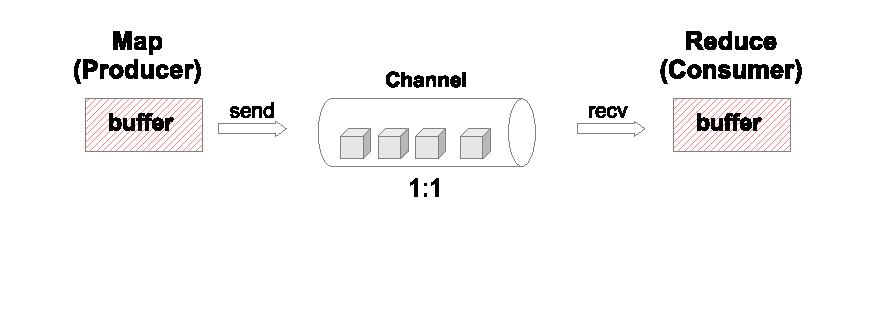
\includegraphics[width=0.4\textwidth]{eps/dmr_channel.eps}
	\caption{Produce-Consume model in SMR}
	\label{fig:dmr:channel}
\end{figure}

%如图所示,这个模型中有两个主要的数据结构:一个map私有buffer pool,其中的每个buffer用于存放发送给对应reduce的数据。一个channel用于mapper和reducer之间数据的传递。
As depicted in Figure \ref{fig:dmr:channel}, in our producer-consumer model, there are two major data structures:
a local \code{buffer} for each map worker is designed to store the intermediate key-value pairs; 
a one-to-one \code{shared-channel} in \myth is used to communicate between map and reduce workers.
With the use of the one-to-one \code{shared-channel}, map worker sends the data to reducer without contenting with other map workers.
When the \code{buffer} threshold is reached,
the map worker will send data in \code{buffer} to the shared-channel and then set the \code{buffer} as empty.
So the \code{buffer} will be reused in the hole Map phase, which saves overhead caused by dynamic memory allocation.
If the \code{shared-channel} is full,  by triggering the \codet{extension} mechanism described in Section 3.3, map worker can continuously work without waiting for the reduce worker to remove the data from the shared-channel.


%When an intermediate key-value pair is generated by the mapper,
%the partition function is used to index the corresponded buffer.
%Once the buffer is determined, 
%the mapper inserts the key-value into the buffer.
%When the buffer threshold is reached,
%the map worker will send data into the buffer to the channel by invoking \code{chan\_send}.
%Then the reduce worker can read record in the channel by \code{chan\_recv}.
%One reduce worker will get key-value from each channel by Round-Robin and 
%merge the key-value pairs to the global buffer.

%Figure.\ref{fig:dmr:pc-model} shows producer-conusmer model in our \myds.  
%There is a one to one channel between map worker and reduce worker, 
%avoiding the contention of multiple map workers.
%When the buffer is full, map worker send the buffer to channel, 
%at the same time, 
%reduce worker receive data from channel, and copy it to local buffer.
%on the other hand,
%we use the a special mapping to allow producer and consumer parallelization effectively, 
%without waiting when the queue is full, or malloc and free operations.
%When the local buffer is full,
%it send the data to channel and then use the buffer again.
%That means map no need wait and there is no many malloc and free operations.
%Figure\ref{fig:dmr:pc-model}
%Thus, this parallelization effectively decouples the behavior of proucer and conusmer, and allows them to be overlapped 
%without many malloc and free.
%In Section\ref{} we have present the design of Channel.


%如同Phoenix, 默认情况下,buffer使用hash table来实现,事实上,在我们的模型中,使用array来实现具有更好的性能。下面的章节会详细解释原因。
In fact, there is a local buffer pool for each map worker, in which each buffer is used to store key-value  pairs which will be sent to a corresponded reducer.
%According to the partition function, the map worker can index which buffer to insert the key-value.
When a key-value pair is generated by the map worker, the partition function is invoked to index the corresponded buffer.
Once the buffer is determined, the map worker will insert the key-value pair into this buffer.
In default, the buffer in \myds is a hash table which is similar to Phoenix's buffer.
We also provide an array buffer implementation for \myds and we will detail the advantage of array buffer in next subsection.







%{\color{gray}
%In the shared-memory model, a region of memory that is shared
%by cooperating processes is established. 
%Processes can then exchange information 
%by reading and writing data to the shared region.
%Shared memory can be faster.
%since in shared-memory systems, system calls are required only to establish shared-memory regions. 
%Once shared memory is established, all accesses are treated
%as routine memory accesses, and no assistance from the kernel is required.
%}
%%SPMC区域的建立
%Interprocess communication using shared memory requires communicating
%processes to establish a region of shared memory. Typically, a shared-memory
%region resides in the address space of the process creating the shared-memory
%segment. Other processes that wish to communicate using this shared-memory
%segment must attach it to their address space. 
%
%%SPMC区域的使用,对应buffer
%To allow producer and consumer processes to run concurrently, we must have
%available a buffer of items that can be filled by the producer and emptied by
%the consumer. This buffer will reside in a region of memory that is shared by
%the producer and consumer processes.(http://bulk.fefe.de/scalability/)



\subsection{Buffer Design and Optimize}
Mites \cite{mao2010metis} shows that the organization of intermediate data is critical to the performance of many MapReduce applications.
%since the entier body of intermediate data must be reorganized between the Map and Reduce phase:
%Map produces data in the same order as the input, while Reduce must consume data grouped by key.\cite{mao2010metis}
%And in a data center, it  
In cluster, it is the network bandwidth dominates the performance, but on multicore system the performance is dominated by the operations on the  data structure that holds intermediate data.
Defaultly, buffer in \myds is a hash table (Figure \ref{fig:dmr:hash-buffer}(a)), in which each entry is a pointer, pointing to key array sorted by key.
%\myds stores the key-value pairs in an array sorted by key.
If the hash table has enough entries, collisions will be rare and the key arrays will be short,
so that lookup and inserting will cost O(1), which is an attractive quality for workloads.
%The hash table's O(1) lookups make it particularly attractive for workloads with many repeated keys.


\begin{figure}[!h!t]  
	\centering
	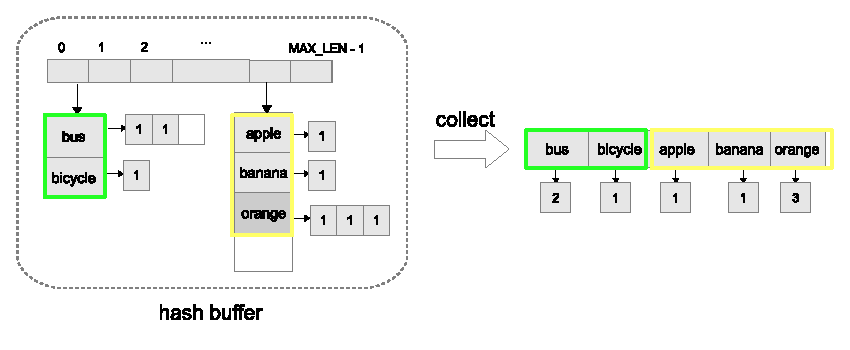
\includegraphics[width=0.5\textwidth]{eps/dmr_hash_buffer.eps}
	\caption{hash buffer and gather}
	\label{fig:dmr:hash-buffer}
\end{figure}
%the element is indexed by the hash value of the key.
%Inside each entry of a hash table,


%{\color{gray}(the reduce operator is immediately applied
%	to that pair based on the local container. This process is
%	performed using a combiner.)}

Based on \myth, our producer-consumer model  requires that data sent to the channel should be a contiguous block of memory.
Since the key arrays in the hash buffer is scattered, which implies that all of the key arrays should be gathered together before sending them to the channel.
This issue can be solved by copying these scattered key arrays out  from the hash buffer and then inserting them into a new contiguous memory region (Figure \ref{fig:dmr:hash-buffer}(b)).
This extra copy is unfortunate and time-consuming.
Furthermore, the hash buffer also requires frequent allocations and deallocations of memory for key and value, and simultaneously couples with the data structure creation and destruction, which will 
negatively affects performance.

%为了提高效率,避免group阶段产生的开销,我们试图改进buffer的hash实现,它不再采用原来 Phoenix 中的 hash 表的组织方式,而是采用更简单的 array,map worker 产生的 key-value只需追加到 array 中即可,无需排序。

%The buffers are initially sized to a default value and then resized dynamically as needed.
To avoid the time-consuming gather in hash buffer, we  implement an easy-to-use array buffer, and the map worker could store its output by appending  key-value pairs to array buffer.
The array buffer is initially sized to a default value, and it can be reused in the hole of Map phase.
%After sending the data of buffer, 
The map worker will indicate the buffer as empty at the end of a sending, but will not free the memory until all map jobs have been finished.
This manner avoids the expensive costs of memory allocation and deallocation as well as the data structures construction and destruction.
Above all, unlike hash buffer, the array buffer is a contiguous memory block, it not have to gather key-value pairs before sending.
The experiment results show that the array buffer is more effective than the hash buffer for some applications that likely have abundant key-value pairs, such as word\_count (Section 5).

% For the array buffer implementation and no combiner in map phase,
% Map just need to . Thus, this technique is more effective
% for array buffer implementation than hash table buffer
% implementation.

%{\color{gray}(A related problem is that eager pipelining moves some of the
%sorting work from the mapper to the reducer.
%Recall that in the
%blocking architecture, map tasks generate sorted output: all the re-
%duce task must do is merge together the pre-sorted map output for
%each partition. In the eager pipelining design, map tasks send out-
%put records in the order in which they are generated, so the reducer
%must perform a full external sort. Because the number of map tasks
%typically far exceeds the number of reduces [4], moving more work
%to the reducer can degrade performance.
%)}




%applications of different buffer as table\ref{diff-buf}
%\begin{table}[]
%\centering
%\caption{My caption}
%\label{diff-buf}
%\begin{tabular}{|l|l|}
%\hline
%\multicolumn{2}{|l|}{\textbf{best buffer of applications}} \\ \hline
%\textbf{application}           & \textbf{buffer}           \\ \hline
%histogram                      & array                     \\ \hline
%word count                     & array                     \\ \hline
%linear regression              & hash                      \\ \hline
%string match                   & hash                      \\ \hline
%pca                            & hash                      \\ \hline
%\end{tabular}
%\end{table}


